\chapter{Boosted Physics as an Experimental Tool}
\label{ch:boost}
\label{sec:RNjets}
Having covered the theory of the standard model, LRS extensions, and the \CMS experiment at the \LHC in broad strokes, it is now important to focus in on cutting-edge techniques in boosted physics that make parts of this analysis possible. 

LRS models do not give any suggestions for the \NR and \WR mass relationship. In the lighter \NR phase-space, the neutrinos will be produced with large transverse momentum, called ``boost''. Therefore, searches where the \NR is much lighter than the \WR, though heavy in standard model comparison, must be performed in tandem with past searches where \NR is assumed of similar mass to the \WR. A boosted \NR search is challenging, as the three decay products of the \NR are no longer likely to be individually isolated, as traditional \WR searches assumed. The specific ratios of the mass of the \WR and \NR where this object overlap from boost becomes significant is shown in Fig.~\ref{fig:NRjet}. A more detailed discussion on the physics of \NR ``jets'' can be found in \cite{nrjets}.
\begin{figure}[!tp]
    \centering
    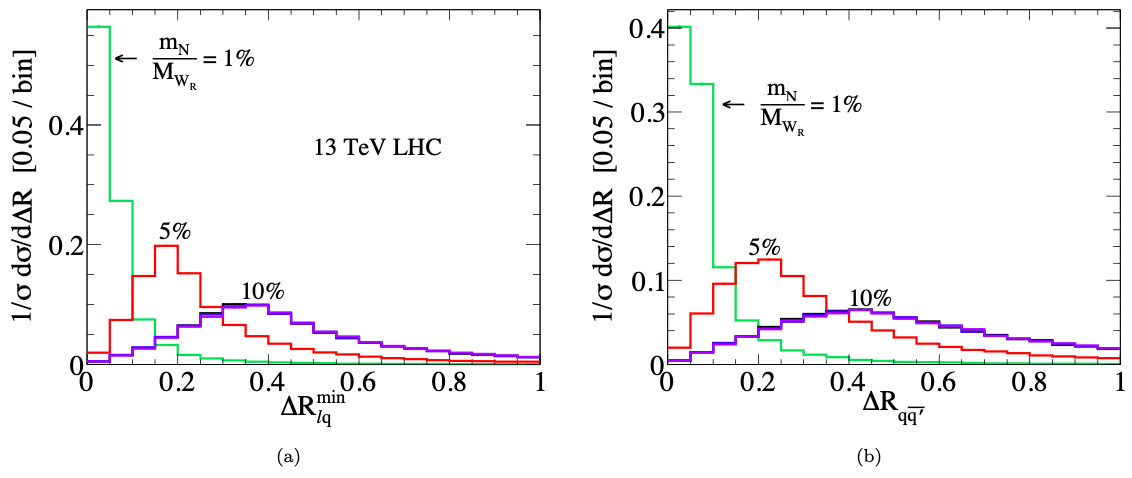
\includegraphics[width=\textwidth]{figures/nrjet_paper_plot.png}
    \caption[
        %short caption
        Angular separation of boosted \NR decay products
    ]    
    {
        Minimum angular separation of the lepton and a quark from \NR decays (a) and the separation of the two quarks in the \NR decay (b) are shown. Three different mass ratios of the \NR and \WR are shown in each. For jets reconstructed with $\Delta R = 0.8$, virtually all of these \NR decays would have their quarks and lepton found within the jet\cite{nrjets}. As the \NR mass decreases, the decay products begin to fit within the $\Delta R = 0.4$, the smaller jets used in this analysis.
    }
    \label{fig:NRjet}

\end{figure}

The substructure of jets made from boosted decay objects is the subject of ongoing study at the \CMS and the \LHC. The ability to distinguish multiple objects within jets allowed \CMS to publish the groundbreaking observation of the Higgs to bb decay in 2018. This thesis adapts some of these techniques to expand the mass limits on the \WR and \NR where the \NR forms a merged jet. These are discussed in the following sections.

\section{Boost}
Before delving too deeply into the algorithms used to study jet substructure, it's important to take a step back and cover the basics of boost as a special relativity concept and one of the more simple examples of it at \CMS, the decay of a boosted particle into two parts.
\subsection{Special Relativity}
Boost is a concept coming from special relativity. A basic premise of special relativity is that the speed of light should always be observed as constant, regardless of the relative motion of the observer with the respect to the emitter.
The consequences of this, time dilation and length contraction, are observed as particles generally travel close to the speed of light. Distances parallel to the motion of the particles are measured shorter in the lab frame than they would be measured with the particles at rest. Both time dilation and length contraction are proportional to $\gamma$, which is called ``the boost''. The boost can be written as a function of the speed of an object and the speed of light, or in natural units is the ratio of the energy over the rest mass of a particle:

\begin{equation}
    \label{eq:lengthcontraction}
    \gamma
    =
    E / m_{0} .
\end{equation}
Using $\gamma$, the length contraction and time dilation can be defined as
\begin{equation}
    \label{eq:lengthandtime}
    L
    =
    L_{0} / \gamma ,
    \  
    t
    =
    \gamma t_{0} .
\end{equation}
 A measured proper length $L_0$, or the length measured when at rest, is divided by $\gamma$ and becomes equal to lab measured value. The proper time $t_0$ is dilated by the factor $\gamma$. However, distances perpendicular to the motion are not affected.

\subsection{Boosted Two-Body Decays}
The effect of special relativity contracting only the parallel coordinates can have significant effects on a process as viewed in the lab frame. As an example, consider a process like \higgstobb.  Considered at rest, the two decay quarks will travel back-to-back to conserve momentum. As can often happen at the \LHC, the Higgs boson may be produced with significant momentum, and while its decay particles are produced back-to-back in the Higgs frame of reference, they are additionally travelling in the direction of the Higgs in the lab frame. This results in two quarks which travel in the same direction in the lab frame.

\begin{figure}[!tp]
    \centering
    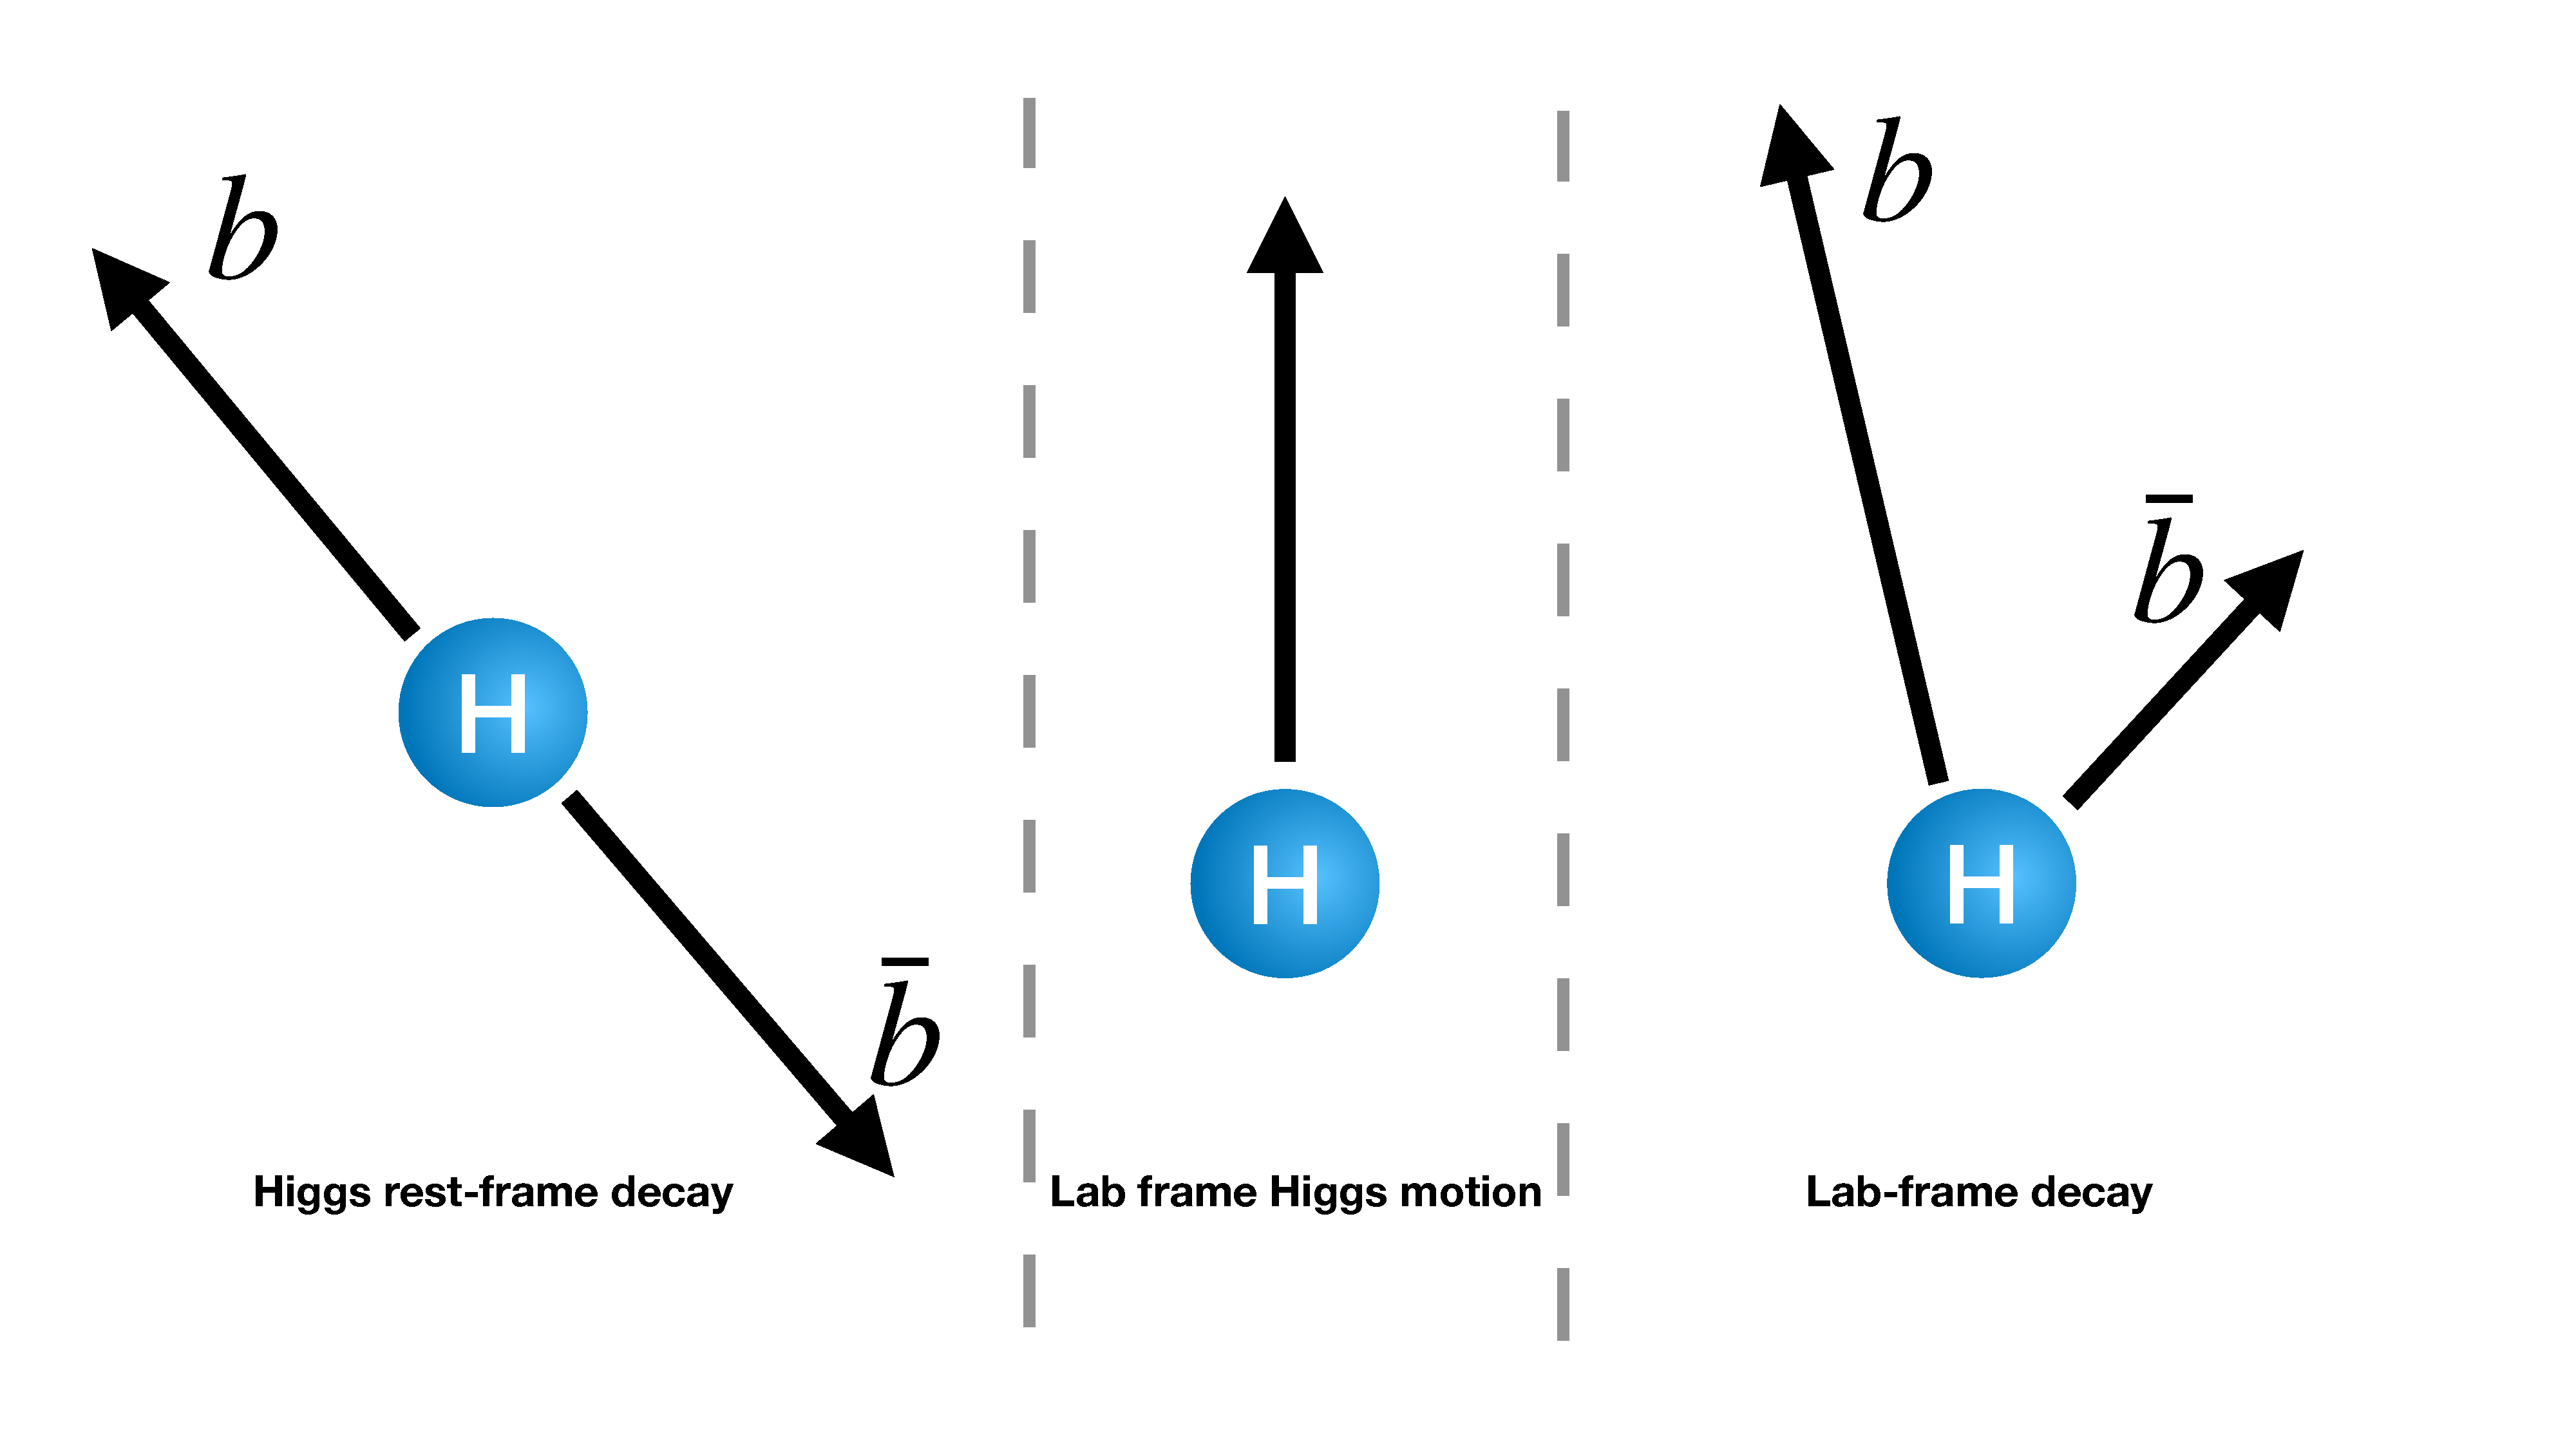
\includegraphics[width=\textwidth]{figures/twobodydecay.pdf}
    \caption[
        %short caption
        Boosted two-body Higgs boson decay
    ]    
    {
        On the left, a back-to-back decay of the Higgs to two b quarks is shown. With significant momentum of the Higgs, this process is observed differently in the lab frame of reference, shown on the right.
    }
    \label{fig:twobody}

\end{figure}

When the momentum of the particle undergoing decay is larger than its rest mass, the momentum the decay particles get from the boost will exceed the momentum received from the decay energy itself. In this case, and as is shown in Fig.~\ref{fig:twobody}, the decay particles will both travel in the direction of the initial particle, and in the lab frame appear closer and closer to each other as the boost continues to increase. At \CMS, a rule of thumb in a two body decay is that the angular separation between the particles proportional to the mass and transverse momentum of the initial particle:
\begin{equation}
    \label{eq:lengthandtime}
    \Delta R
    \approx
    2m / \pt .
\end{equation}

\section{The ``impossible'' Higgs decay}
The search for the Higgs boson decaying to two b-quarks in \CMS is a landmark study for boosted physics and provides a perfect frame-of-reference to discuss boosted techniques in.

The standard model Higgs boson couples to fermions according to their mass. With the heaviest fermion available for Higgs decay being the b-quark, the 58\% of Higgs will decay to pairs of these quarks. The two leading discovery channels for the Higgs, however, were the \higgstoZZtollll and \higgstogammagamma gamma decays which make up less than half a percent of Higgs decays, far less frequent than a decay to b quarks \cite{pdg2018}. From the beginning of the design of \CMS and the LHC, it was not expected to be possible to even observe \higgstobb as the rate at which everyday QCD processes can produce pairs of b quarks is vastly higher than the Higgs process.

As the collision energy and luminosity of the \LHC increased in Run II, a new technique for analyzing Higgs decays emerged. Some small fraction of Higgs are produced in the \LHC with significant transverse momentum. This Higgs momentum, or ``boost'', collimates the decay products of the Higgs in the lab frame making the signature distinct from a QCD process. A QCD process is very unlikely to produce two relatively collinear heavy quark pairs with significant momentum. While the chance of a boosted Higgs is also low, the ratio of signal to background rises dramatically with the requirement of a boosted object. The new challenge then, is distinguishing two individual b quarks pushed together into a single jet by the boost of the Higgs. For full details on the boosted \higgstobb analysis see \cite{boostedHiggsTobb}.

\section{Jet Algorithms}
\label{sec:jetalgorithm}

As discussed in Section \ref{sec:QCD}, quarks and gluons exiting a hard collision at \CMS produce a multitude of soft collinear QCD radiations. The hadronization process occurs extremely rapidly, and by the time the hadronized particles have travelled outside the beamline, they have formed a ``jet'': several energetic hadronic particles travelling roughly collinearly. As the jet of hadrons continues through the detector, each is measured in different ways according to its specific quark composition. In order to capture the kinematics of the original quark or gluon involved in the hard process, all of the QCD radiations must be associated and summed until all of the parts of the hadronization have been combined.

\CMS generally uses a variant of the Cambridge-Aachen jet algorithm called \antikt. Each type of jet algorithm tries to organize all the particles observed in the detector into a set of jets, and has advantages and disadvantages dependent on a large variety of situations. 

%

\subsection{The \antikt Algorithm}
Particle flow (PF) jets are created using a jet algorithm to associate individual PF particles. The two key relations in this algorithm are:
\begin{equation}
    d_{ij} = \mathrm{min}\left(k^{-2}_{ti},k^{-2}_{tj}\right)
    \frac{\Delta_{ij}^{2} }{R^{2}},
\end{equation}
\begin{equation}
    d_{iB} = k^{-2}_{ti},
\end{equation}
where:
\begin{equation}
\Delta^{2}_{ij} = \left(y_{i} − y_{j}\right)^{2} + \left(\phi_{i} − \phi_{j}\right)^{2}.
\end{equation}

The first distance relation $d_{ij}$ is computed between every particle or proto-jet in the event. The second distance $d_{iB}$ is calculated between each proto-jet and the beam. The reconstruction begins by clustering together the closest pair, and continues until every object is included. For instances where $d_{iB}$ is the closest, the jet is removed from consideration for further clustering.

As an example to understand the behaviour of the \antikt algorithm, consider an event with a few well-separated hard particles with transverse momenta $k_{t1}, k_{t2}, . . .$ and several softer particles. The $d_{1i} =\mathrm{min}\left(1/k^{2} , 1/k^{2} \right)\Delta^{2}_{1i} /R^{2}$ between the first hard particle and one of the soft particles, $i$, is determined by the transverse momentum of the hard particle and the $\Delta_{1i}$ separation. The $d_{ij}$ between similarly separated soft particles will be much larger than $d_{1i}$. As a result, soft particles will tend to cluster with the hard particles in the event instead of forming clusters with each other. If a hard particle has no hard neighbours within a distance $2R$, then it will simply accumulate all the soft particles within a circle of radius $R$, and form a conical jet.

In the case where a second hard particle is present and $R < \Delta_{12} < 2R$ two hard jets will form, but it will not be possible for both to be perfectly conical. If one of the jets has significantly more $k_t$, that jet will be conical and the other jet will only be partly conical, missing the soft radiation overlapping with the higher $k_t$. If the two jets are roughly equivalent in $k_t$ neither will be completely conical and the overlap region will be divided between the two. This boundary region is defined by $\Delta R_{1b}/k_{t1} = \Delta R_{2b}/k_{t2}$ \cite{AK_jets}.

%The true separation of all of the hadronization particles is assumed to be independent of their energy. This assumption is successful only when the jet initiator is not boosted transversely.

\subsection{Jet Boost}

Looking at Cambridge-Aachen algorithms broadly, one algorithm assumption is important to revisist when studying boosted objects. The \antikt searches to combine particles within a defined maximum size cone in \etaphi~space. Particles close in momentum and position are iteratively combined together within the cone. These particle pairs are then combined with each other and so on, until all well associated particles have been clusters (and those clusters clustered) to make a single jet.

This process works well the original partons come from an interaction approximately at rest transversely in the detector. Significant transverse boost of the production frame additionally collimates the hadronization in the lab frame, resulting overlapping jets. To combat this, boosted physics searches use larger cone size jets to collect all the particles in a region of the detector which could be associated, for example, with the \higgstobb. These ``fat'' jets are then reclustered into small jets, often two or three, to distinguish sub-components of the jet more tightly associated with each other than the rest of the jet. 
%Two b-quark similar clusters within a jet being the most important criteria for the \higgstobb analysis.   

\section{Techniques in Boosted Physics at Hadron Colliders}

To leverage the kinematic uniqueness of boosted systems significant advancements in techniques have arrived in recent years for the study of jets formed from particles seen as a merged together as a result of their boost.

\subsection{Jet Substructure}

%Jet algorithms used in particle physics experiments like \CMS or \ATLAS are focused towards collecting all of the particles from a single quark or gluon.  There is, however, a significant amount of information that can be understood by looking at scales smaller than the size of jets reconstructed at \CMS. While a typical jet at \CMS is reconstructed with a size of \ensuremath{R_{cone} = 0.4 \| 0.8}, these jets can be re-clustered into smaller pieces.  A jet produced from a single quark may not have much interesting information at a finer scale, however, top quark jets, where multiple decays occur in-flight, or jets formed by the merger of multiple distinct objects may have interesting structural components.  
Several different techniques are used to study the constituents of ``fat'' jets in boosted physics. N-subjettiness is used to determine how many tightly associated subclusters a fat jet might have, key for identification of \bbbar jets in the boosted Higgs analysis. The techniques used in this analysis are lepton subjet fraction (LSF) and soft-drop mass and are discussed further below.

\subsubsection{N-subjettiness}

N-subjettiness is based on reclustering the components of a large jet into multiple smaller jets and then evaluating whether the subcluster splittings are natural or forced. Heavy \QCD jets, which can spoof interesting physics, like a hadronically-decaying electro-weak boson, will have many energetic components all travelling roughly collinearly.  A hadronic decay of a Higgs, however, will have two adjacent b-quark jets and little else.

In order to distinguish between a jet of many approximately equally energetic components which can all be associated, and a jet with two distinct clusters of particles, N-subjettiness defines a variable $\tau_{N}$ which can be calculated for different numbers of subjets, $N$. The variable $\tau_{N}$ can be thought of as a measure of the ``cost'' to associate subclusters, measured in position and momentum space. Generically, $\tau_{N}$ is calculated as:

\begin{equation}
    \label{eq:nsubjettiness}
    \tau_{N}
    =
    \frac{1}{d_{0}}\sum_{k} {p_{T,k} \mathrm{min} \left\{\Delta R_{1,k}, \Delta R_{2,k},\cdots,\Delta R_{N,k} \right\} } .
\end{equation}

A sum over all particles ($k$) in the larger jet is performed, comparing each to the kinematic centers of a chosen number of subclusters. For each particle, its momentum is multiplied by the $\deltaR$ of the closest subcluster center.  For only one jet cluster, $\tau_{N}$ is simple to calculate:
\begin{equation}
    \label{eq:tau1}
    \tau_{1}
    =
    \frac{1}{d_{0}}\sum_{k} {p_{T,k} \Delta R_{1,k}} .
\end{equation}
For the case where two subclusters are considered, the closest of the $\deltaR$ between each particle and the two subcluster kinematic centers is taken. 
\begin{equation}
    \label{eq:tau2}
    \tau_{2}
    =
    \frac{1}{d_{0}}\sum_{k} p_{T,k} \mathrm{min} \left\{\Delta R_{1,k}, \Delta R_{2,k}\right\}  .
\end{equation}
The ratio of $\tau_{N}$ for different values of N is taken to compare the relative ``cost'' of different subcluster arrangements. In the \higgstobb study, the most important ratio is  $\tau_{2}$/ $\tau_{1}$, called $\tau_{21}$. A number closer to zero points a more natural di-cluster than a single jet clustering. The discriminating power of $\tau_{21}$ to distinguish between an electroweak boson's hadronic decay, and a \QCD jet is shown in Fig.~\ref{fig:nsubjettiness}.

\begin{figure}[!tp]
    \centering
    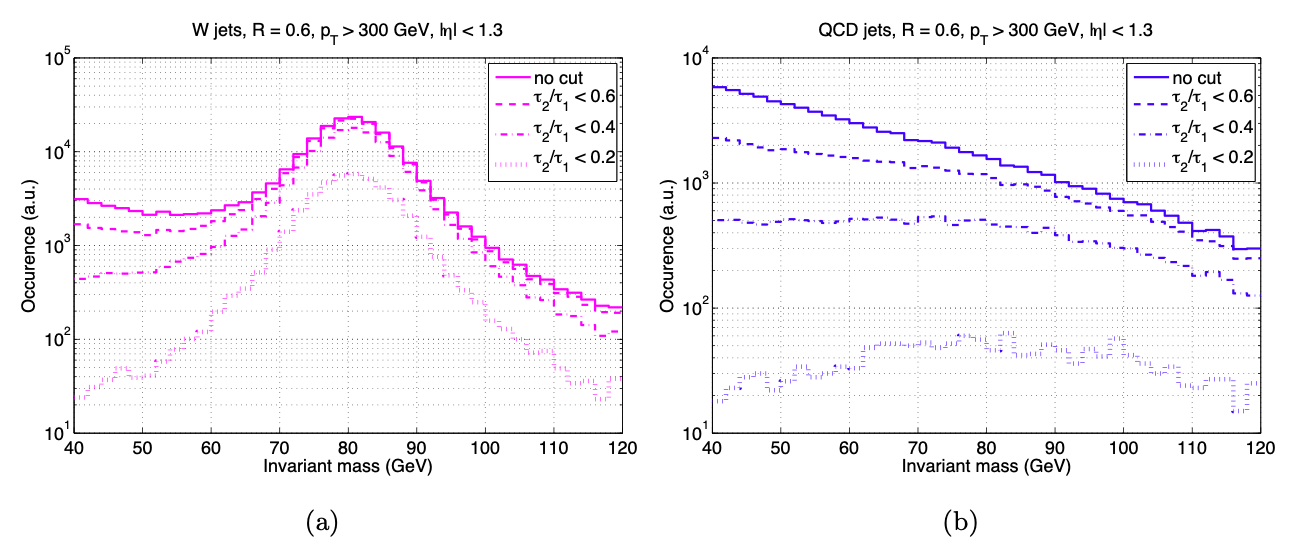
\includegraphics[width=\textwidth]{figures/Nsubjettiness_paper.png}
    \caption[
        %short caption
        N-subjettiness performance \LHC
    ]    
    {
        N-subjettiness performance can be seen in (a) with W jets and (b) QCD jets.  Tighter cuts on the \ensuremath{\tau_{2}/\tau_{1}} ratio yield better W mass peaks \cite{Nsubjettiness}.
    }
    \label{fig:nsubjettiness}
    
\end{figure}
    
This analysis studied the benefits of various N-subjettiness ratios, and did not find any to be particularly helpful for discriminating signal and background. Which suggests that the leading backgrounds for the analysis have a similar topology to the boosted neutrino decay. The QCD background which is important in \higgstobb is suppressed in this analysis by requiring a lepton within the fat jet cluster. We therefore move to an important tool for lepton identification in the boosted regime. A complete discussion of N-subjettiness is found in \cite{Nsubjettiness}.


\subsubsection{Lepton Subjet Fraction}

\label{sec:lsf}

Lepton signals at hadron colliders like the \LHC serve as clear indicators of interesting physics.  While quarks and gluons play large roles in interesting particle physics, hadron colliders produce them in over abundance.  The events of quarks and gluons in the final state, hadronizing to jets, make up the vast majority of the interactions at the \LHC and make distinguishing a specific process of interest challenging. Leptons, on the other hand, indicate an electroweak interaction occured. If that interaction occurred early in the event (rather than as part of a meson decay), it is often a signature of an interesting event.

To select away from meson decay, leptons used in searches for new physics are required to be isolated from other detector signals. A hard electroweak interaction typically kicks its lepton far away from the rest of the interaction, well isolating it. This scenario holds for the resolved version of this analysis, where the \NR and \WR are not moving before decaying, and each particle travels far from the others. When a meson decays, however, the muon will share that meson's momentum, and travel roughly collinear with the hadronic activity associated with the meson, which is part of a jet, The jet, therefore, will often contain leptons from the decay of its charged mesons. The situation where a lepton is travelling along with other jet constituents is similar to when the \NR is boosted. A boosted \NR will produce a muon physically close to the quarks in the \NR decay similarly to the meson decay picture.

In the typical non-boosted analysis, relative momentum isolation is used to remove decay-in-flight leptons. The \ensuremath{p_T} of all particles within a certain size cone are summed and compared with that of the lepton. This is defined as:
\begin{equation}
    \label{eq:relISO}
    \mathcal{R}_{\text{iso}}^{\ell}
    =
    \frac{\sum_{i}p_{T,i}}{p_{T,\ell}},
\end{equation}
The cone size is typically 0.3, and the value of \ensuremath{\mathcal{R}_{\text{iso}}^{\ell}} can be tuned for a particular analysis and often falls within the range 0.1-0.2.
It can be readily seen that the fixed-size cone fails again for boosted objects. In the specific case of the lepton in a \NR jet, it will be momentum-isolated from the two quarks in the \NR decay, but the relative isolation defined in Eq.~\ref{eq:relISO} will fail to identify this. 

To measure the isolation of leptons in boosted jets, a technique called Lepton Subject Fraction (LSF) is used. In this analysis, the selected ``fat'' jet is clustered into three subjets corresponding to the expected number of original constituents (a lepton, and two quarks). Any lepton within the main jet will be clustered into one of the 3 subjets. The relative transverse momentum of the subjet and the transverse momentum of the lepton defines LSF. In the re-clustering, the muon should be too far away in momentum space to be clustered with most of the two quarks' QCD radiation. Therefore, the lepton will be mostly alone in its subjet and the ratio of its momentum to the momentum of entire subcluster will be close to one.
\begin{equation}
    \label{eq:LSF}
    \mathrm{LSF}
    =
    \frac{p_{T,\ell}}{p_{T,sj}}.
\end{equation}
The performance of LSF versus relative isolation is shown in Fig.~\ref{fig:LSFvRelIso} \cite{PHPaperLSF}.

\begin{figure}[!tp]
    \centering
    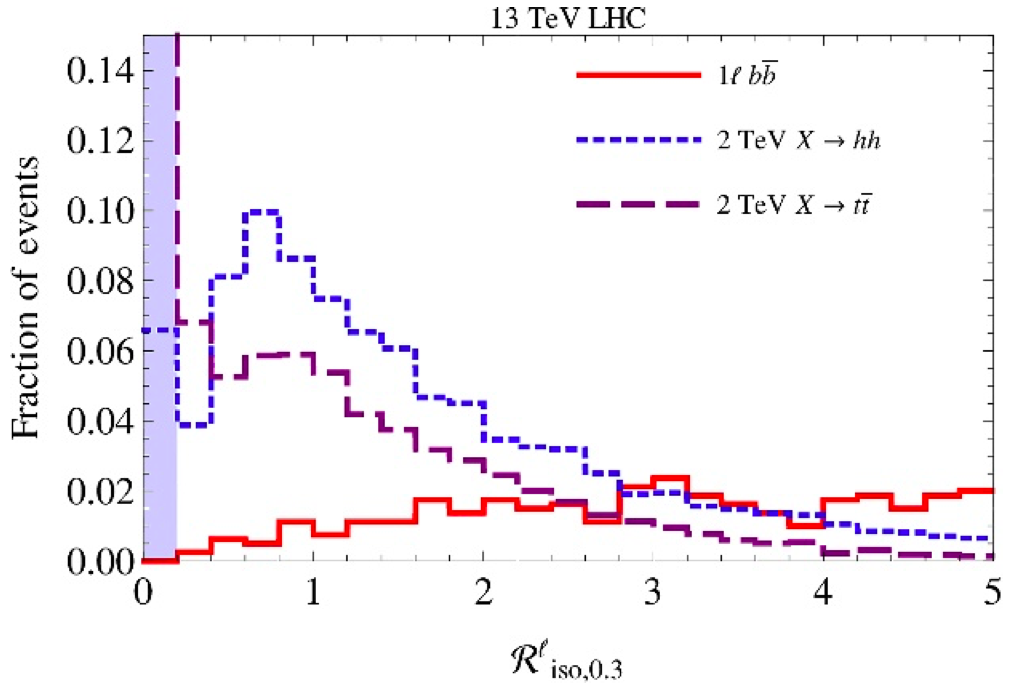
\includegraphics[width=0.6\textwidth]{figures/RelIso0_3.png}
    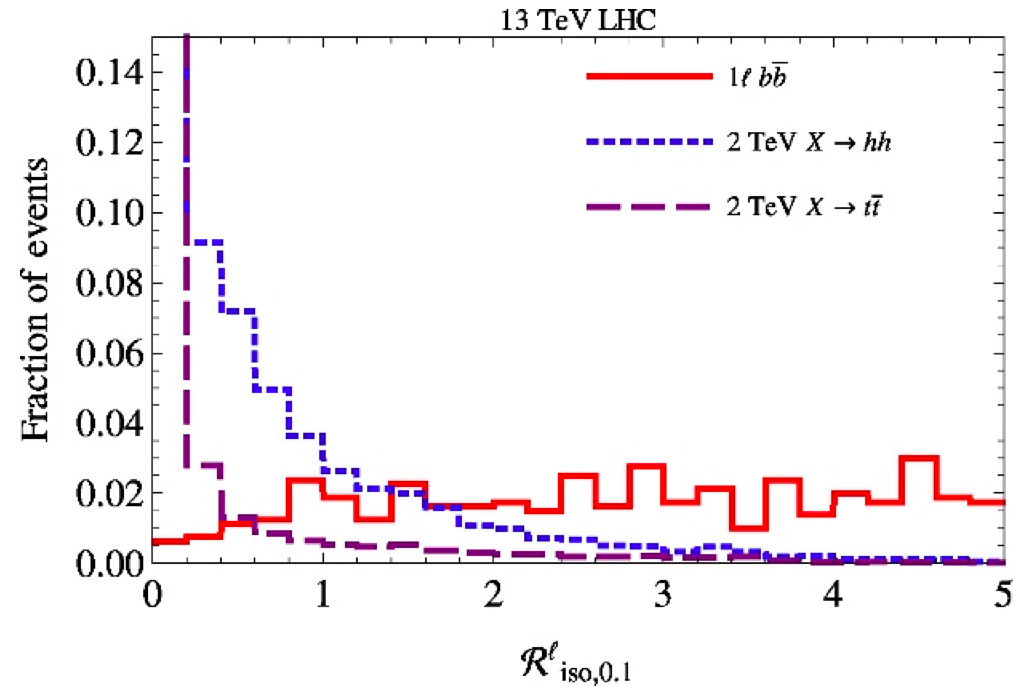
\includegraphics[width=0.6\textwidth]{figures/RelIso0_1.png}
    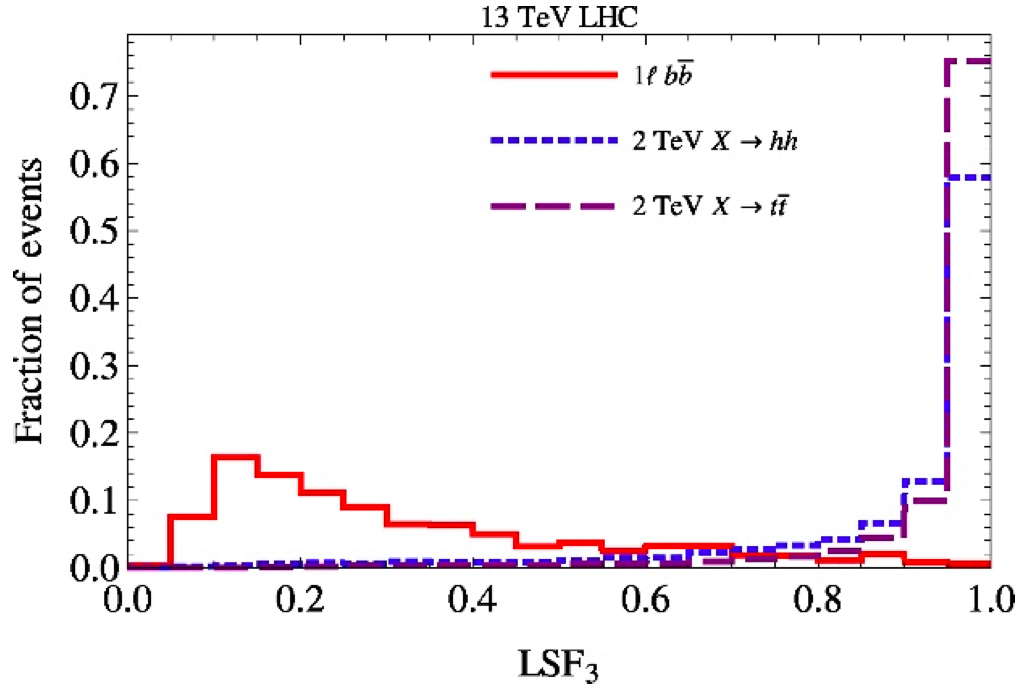
\includegraphics[width=0.6\textwidth]{figures/LSF_paper_plot.png}
    \caption[
        %short caption
        LSF performance compared to relative isolation
    ]    
    {
        From top to bottom, these plots show the performance of a relative isolation cut of 0.3, 0.1, and $LSF_{3}$.  Each shows the behavior for a semi-leptonic \ensuremath{b\bar{b}} and a theoretical \ensuremath{\SI{2}{\TeV}} object decaying to two Higgs or a \ensuremath{t\bar{t}} pair.
    }
    \label{fig:LSFvRelIso}

\end{figure}

\subsubsection{Soft Drop Mass}

\label{sec:softdrop}

At the current \LHC luminosities, multiple events interact and are recorded simultaneously in a bunch crossing. This ``pileup'' of events is problematic for jet measurements. As each jet is constructed, QCD radiation from the pileup and the underlying event will additionally be clustered with the hadronization of interest, or in many cases be made purely of QCD. The soft-drop procedure removes soft, wide-angle radiation in jets. The mass of a jet from QCD contributions tends toward zero after this process while the mass coming from hard radiation remains. 
%This technique is generically called ``jet grooming'' techniques exist. Many techniques exist but, \CMS uses soft drop.

In soft drop, jet constituents are clustered in a pair-based clustering scheme with angular ordering (the Cambridge-Aachen jet algorithm\cite{AK_jets}). The clustering is brought to where there are just two subjets, we can label them as \ensuremath{j_1} and \ensuremath{j_2}.  These are then compared with:
\begin{equation}
    \label{eq:SDmass}
    \frac{min\left(p_{T1},p_{T2}\right)}
    {p_{T1}+p_{T2}}
    >
    z_{cut}\left( \frac{\Delta R_{12}}{R_{0}} \right) ^ {\beta}.
\end{equation}
On the left, the \pt fraction of the lowest subcluster is compared to the angular separation based variable $\left(\frac{\Delta R_{12}}{R_{0}}\right)^{\beta}$ multiplied by a scale, $z_{cut}$.
The behaviour is then tune-able with two variables: \ensuremath{z_{cut}} and \ensuremath{\beta}, depending on the desired response. At \CMS typically \ensuremath{\beta = 0} and \ensuremath{z_{cut} = 0.1}. This simplifies the relationship to:
\begin{equation}
    \label{eq:SDmass}
    \frac{min\left(p_{T1},p_{T2}\right)}
    {p_{T1}+p_{T2}}
    >
   0.1 .
\end{equation}
If this condition is true, neither subcluster is removed from the jet, as they are each considered sufficiently hard.  If the condition is false, the softer subcluster is removed, and the jet is redefined to be the subjet with largest \pt. The two subclusters of this new jet are evaluated and the procedure continues until the two compared subclusters are comparably hard. A cartoon of this process on a \QCD jet and a \NR jet is shown in Fig.~\ref{fig:softdropcartoon}. The soft drop mass procedure is detailed in this paper \cite{SoftDrop}.

\begin{figure}[!tp]
    \centering
    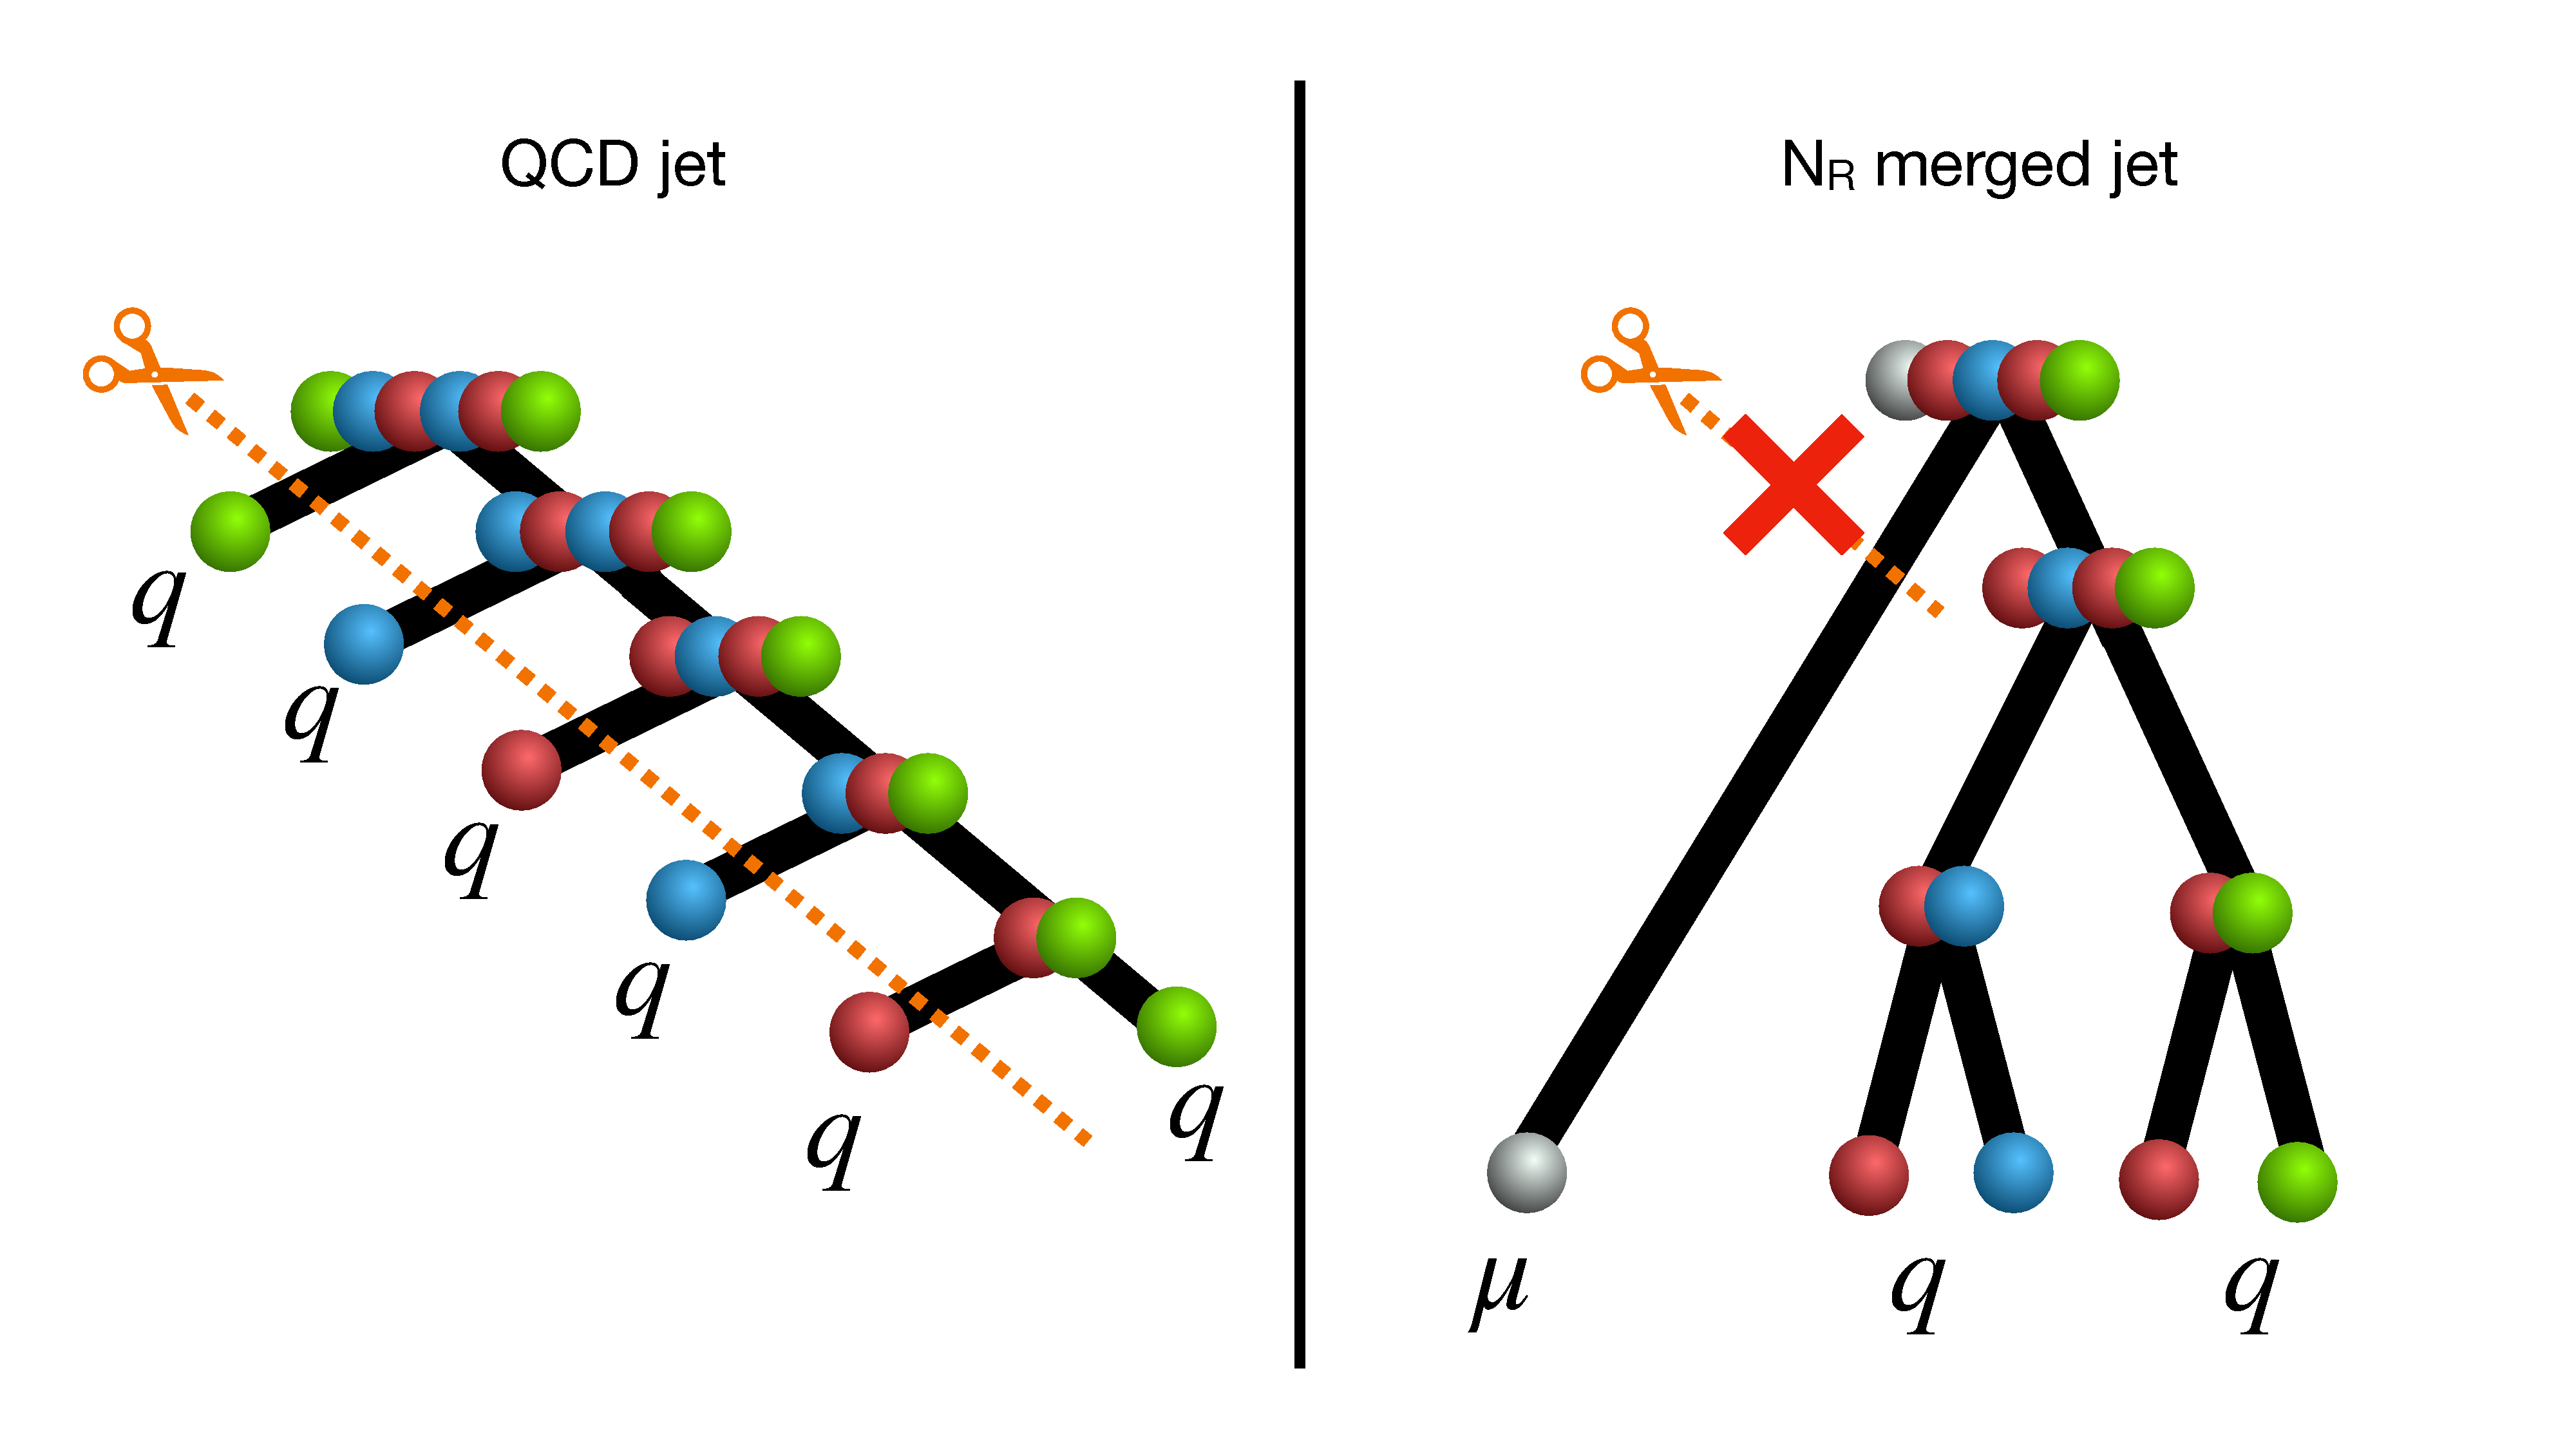
\includegraphics[width=\textwidth]{figures/JetSubstructureComparison.pdf}
    \caption[
        %short caption
        Jet Substructure Comparison
    ]    
    {
       A cartoon of the structure of a QCD jet and a \NR jet is shown on the left and right, respectively. The QCD jet is made up of many soft radiations, each often having much less momentum than the subcluster it is joined with. As the soft drop procedure proceeds, most of the jet is trimmed away. The remaining mass of the jet is minimal. In the \NR case, while there is some color-flow between the two quarks, the muon and the quarks are each hard enough that soft drop does not trim any parts of the jet. The remaining jet mass is close to the \NR mass.
    }
    \label{fig:softdropcartoon}
    
\end{figure}



%\section{Continuing Searches}

%A section to briefly detail some of the more interesting ``state-of-the-art'' boosted physics analyses: Higgs to BB, B2G, etc.